% !TEX root = ../gnss_interference_resistant_thesis.tex
\documentclass[main.tex]{subfiles}

\begin{document}

\subsection{GNSS signalų apdorojimas}

Signalų apdorojimui pasirinkta naudoti atviro kodo programinė įranga
GNSS-SDR \cite{GNSS-SDR11}. GNSS-SDR yra projektas, vystomas
Centre Tecnològic de Telecomunicacions de Catalunya organizacijos,
nuo 2011 metų.

GNSS signalų apdorojimas yra intensyvus procesas,
todėl norint apdoroti juos realiu laiku, reikalingos optimizacijos,
kurios pilnai išnaudotų kompiuterio resursus. Norint išnaudoti resursus,
visus skaičiavimus reikia lygia gretinti, tačiau tai nėra tokia
paprasta užduotis. Ši problema jau yra išspręsta GNU Radio projekto,
todėl GNSS-SDR pasitelkia šį įrankį signalų apdorojimui.

\begin{figure}[h]
    \begin{centering}
    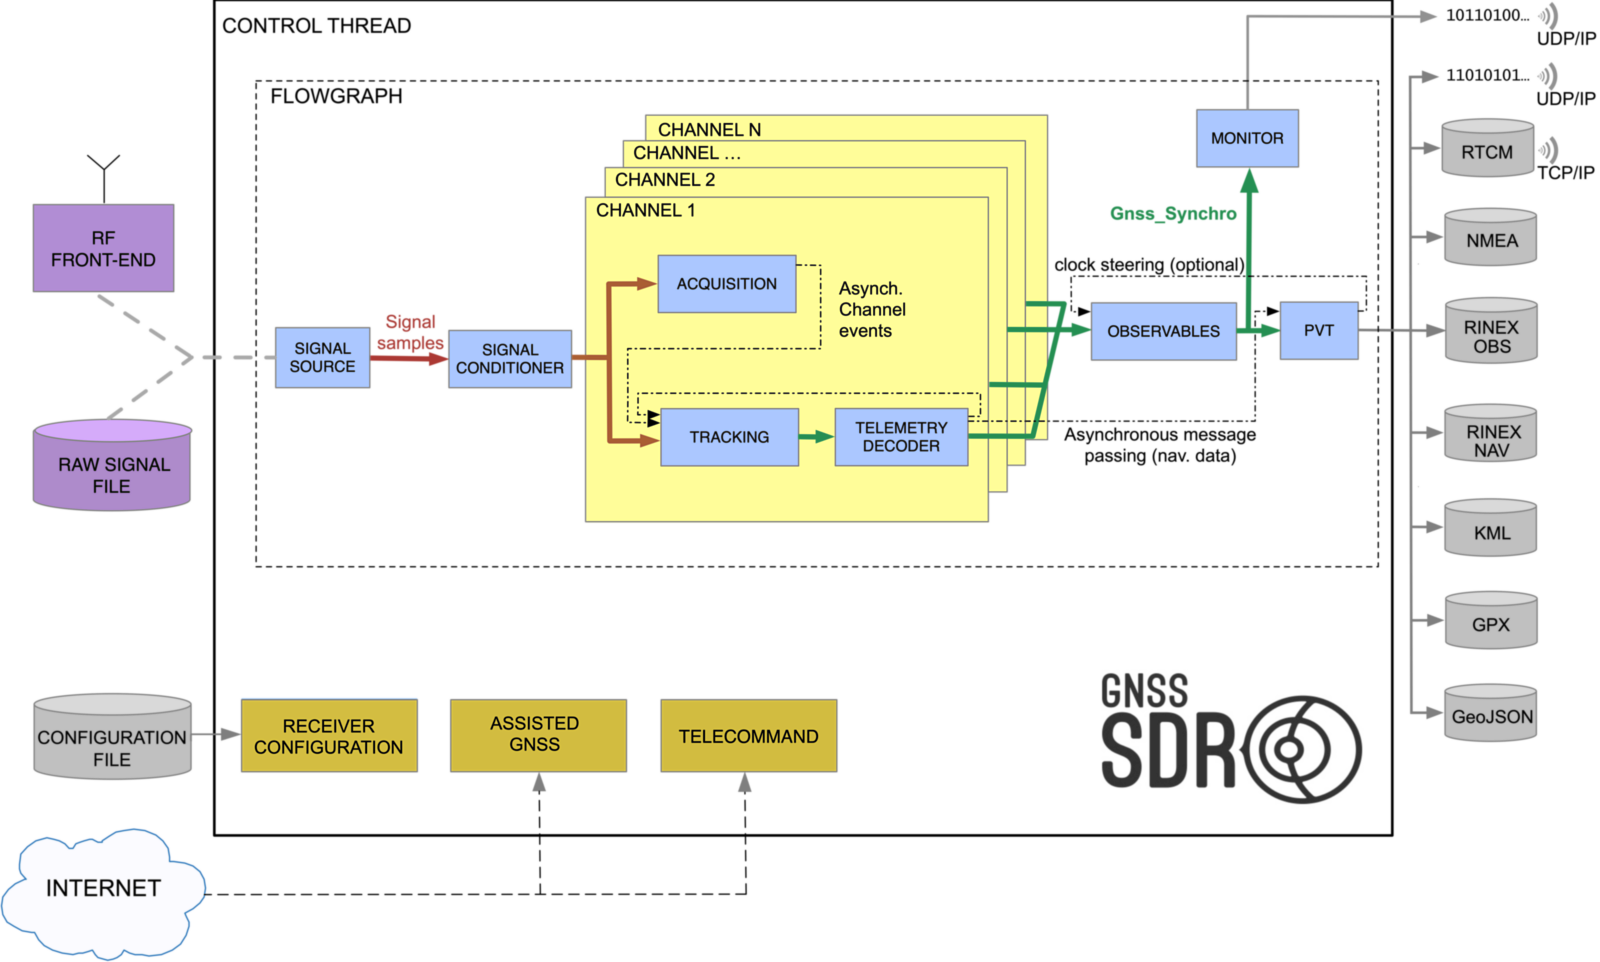
\includegraphics[scale=12.0]{drawings/GeneralBlockDiagram}
    \par\end{centering}
    \protect\caption{\label{fig:gnss_sdr_block}GNSS SDR imtuvo, duomenų apdorojimo schema \cite{gnss_sdr_web}.}
\end{figure}

Signalo apdorojimas prasideda nuo duomenų šaltinio (angl. Signal Source). Duomenų šaltiniu
gali būti arba SDR imtuvas, arba duomenų failas. Dažniausiai SDR imtuvas naudojamas,
kai duomenys yra apdorojami realiu laiku, o duomenų failas, kai duomenis yra apdorojami
vėliau, taip pat duomenų failas yra patogesnis naudojimui kai yra tobulinamas GNSS SDR
kodas, kadangi galima nesunkiai lyginti imtuvo kokybę su tuo pačiu signalu.

Duomenys iš šaltinio turi būti pritaikyti prie vidinio formato. Signalo šaltiniai
dažnai turi skirtingus formatus, skiriasi duomenų rezoliucija, išdėliojimas ir t.t.
Signalo paruošimo (angl. Signal Conditioner) paskirtis yra pritaikyti duomenų šaltinio
formatą prie vidinio formato, naudojamo visuose kituose apdorojimo blokuose.

Kanalai (angl. Channel) yra skirti individualių palydovų paieškai ir sekimui.
Kiekvienas kanalas yra atsakingas už palydovo signalo suradimą (angl. Acquisition),
jį suradus, už jo signalo sekimą (angl. Tracking) ir duomenų dekodavimą (angl. Telemetry
Decoder). Visi kanalai veikia lygiagrečiai, iš pradžių kiekvienam kanalui yra
priskiriamas palydovas kurio jis ieškos ir tada pradedama palydovų paieška.
Aptikus palydovo signalą, pradiniai sekimo parametrai yra perduodami sekimo
blokui, kuris užsirakina ant signalo.

Stebėjimo blokas (angl. Observables) surenka duomenis iš visų kanalų ir atlieka
pseudo atstumo, fazės ir doplerio dažnio matavimus. Iš šių duomenų, galime
rasti imtuvo poziciją, greitį ir laiką, už tai yra atsakingas PVT
(angl. Position-Velocity-Time) blokas. Šis blokas atsakingas už sprendinio
radimą ir rezultato pateikimą skirtingais standartizuotais formatais.

\end{document}
